\documentclass[titlepage]{article} % use option titlepage to get the title on a page of its own.
\usepackage{graphicx}
\usepackage{biblatex} %Imports biblatex package
\bibliography{bibliography.bib}
% \addbibresource{bibliography.bib} %Import the bibliography file
\graphicspath{ {./images/} }
\setlength{\parindent}{0pt}

\title{A Mathematical Framework for “Star Battle” or “Two Not Touch” puzzles}
\date{\today{}}
\author{William Easdown Babb\thanks{GitHub: @weasdown}}

\begin{document}
\maketitle
\section{Introduction}
This document will define a mathematical framework for analysis of Jim Bumgardner’s “Star Battle” puzzles~\cite{krazydad}, which are published in the New York Times as “Two Not Touch” puzzles. These can also be seen in the “Star Battle” Android app~\cite{stars-app}. This document will refer to these puzzles as “Star Battle” puzzles.

We will first define key terminology for the Star Battle puzzles, such as “array” and “cell”. We will then assess how these definitions could enable analysis of more general puzzles, such as those with a different size grid or a different number of stars. Next, we will consider how to analyse a puzzle state to solve it, both purely logically and stochastically.


\pagebreak
\section{Anatomy of a “Two Not Touch” or “Star Battle” puzzle}
This section will define key terminology for the Star Battle puzzles so we can later use these terms when solving them.
An example of a Star Battle puzzle, from the Star Battle app~\cite{stars-app}, is shown in Figure~\ref{fig:example boards}.

% Example puzzles - blank and complete
\begin{figure}[h]
    \centering
    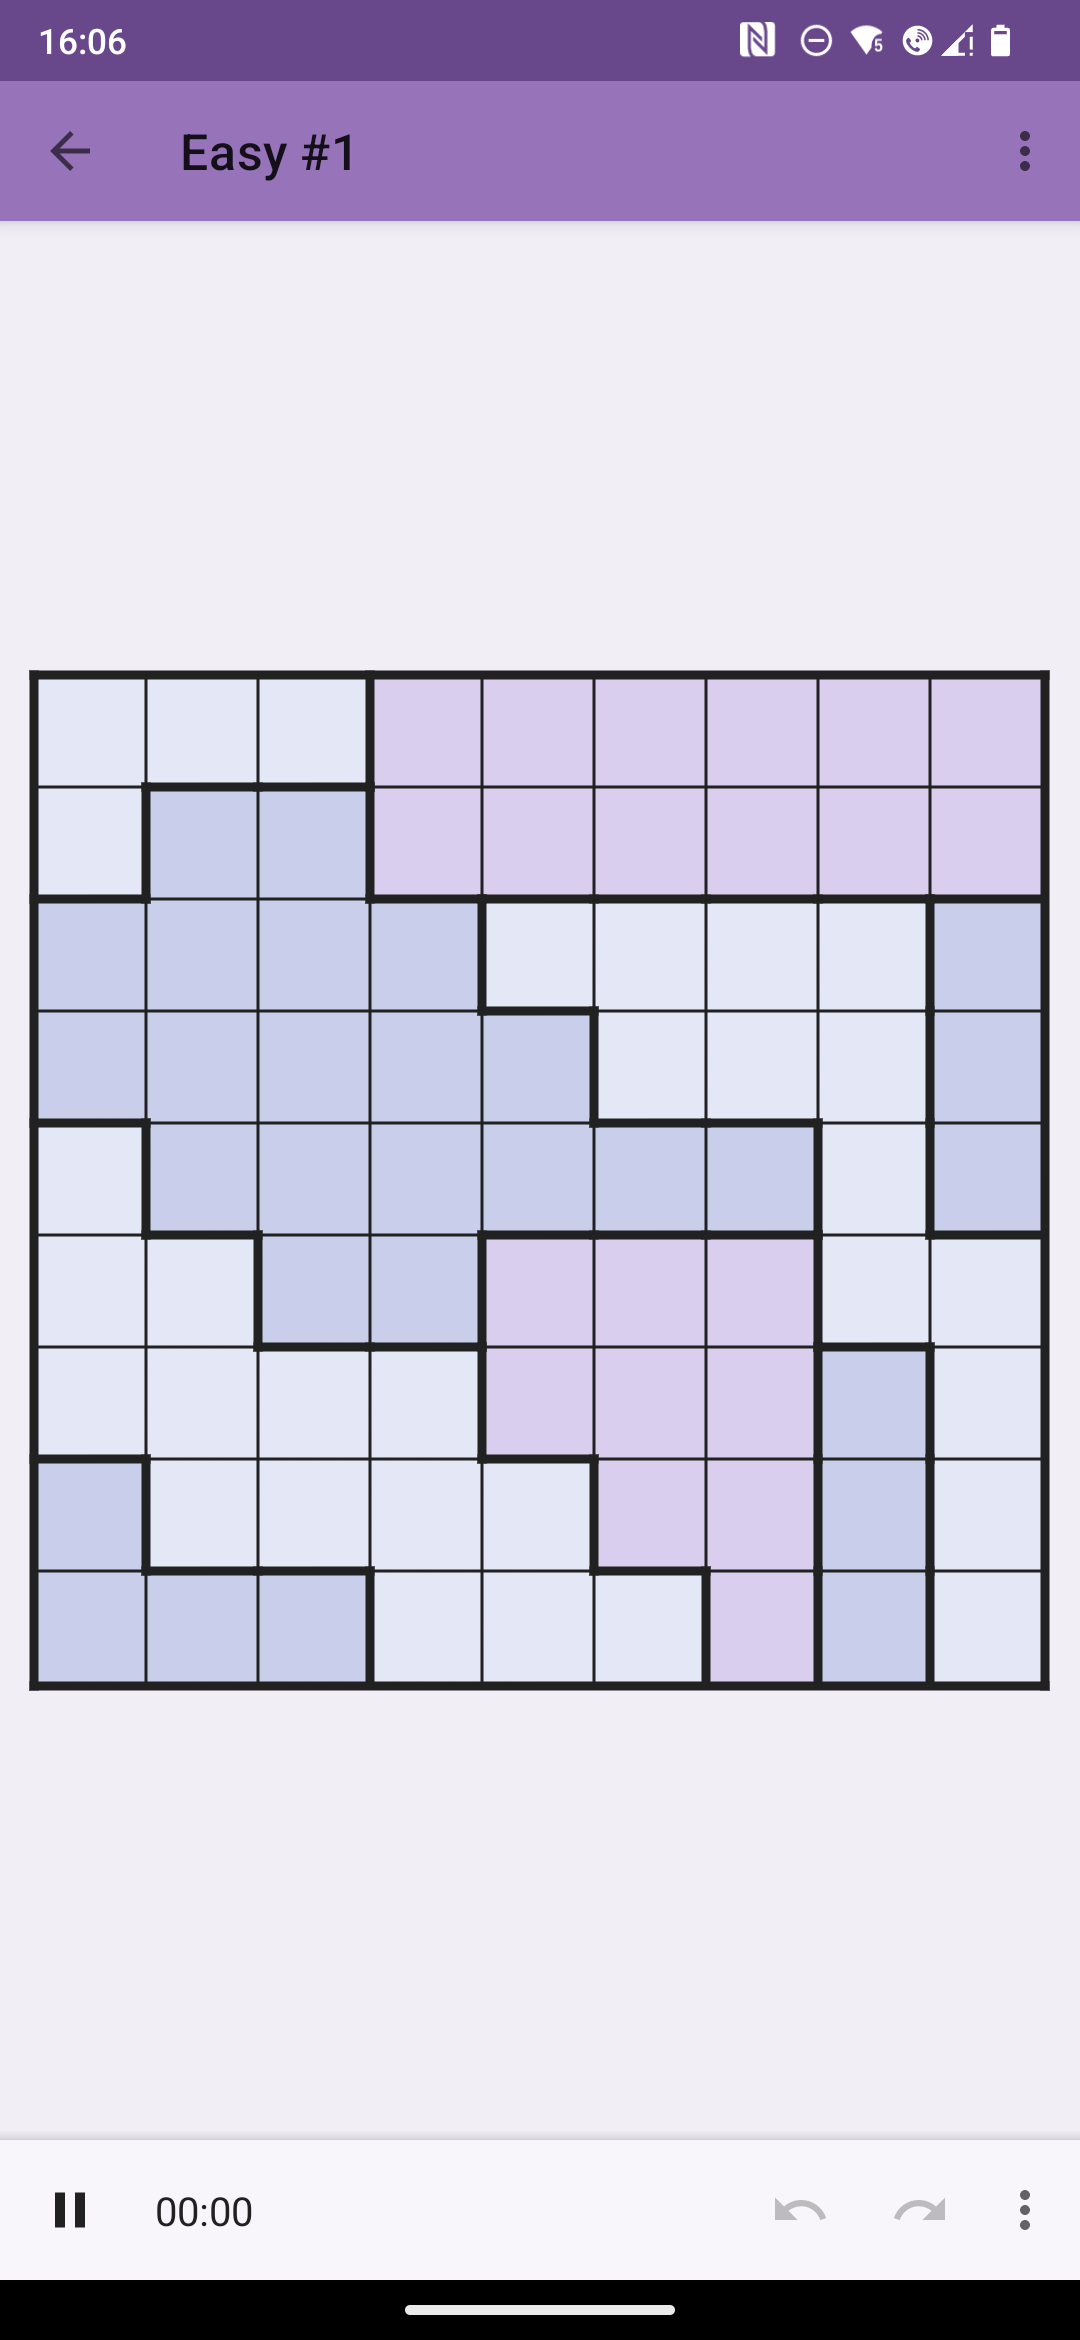
\includegraphics[height=12cm]{Easy_1_blank.png}
    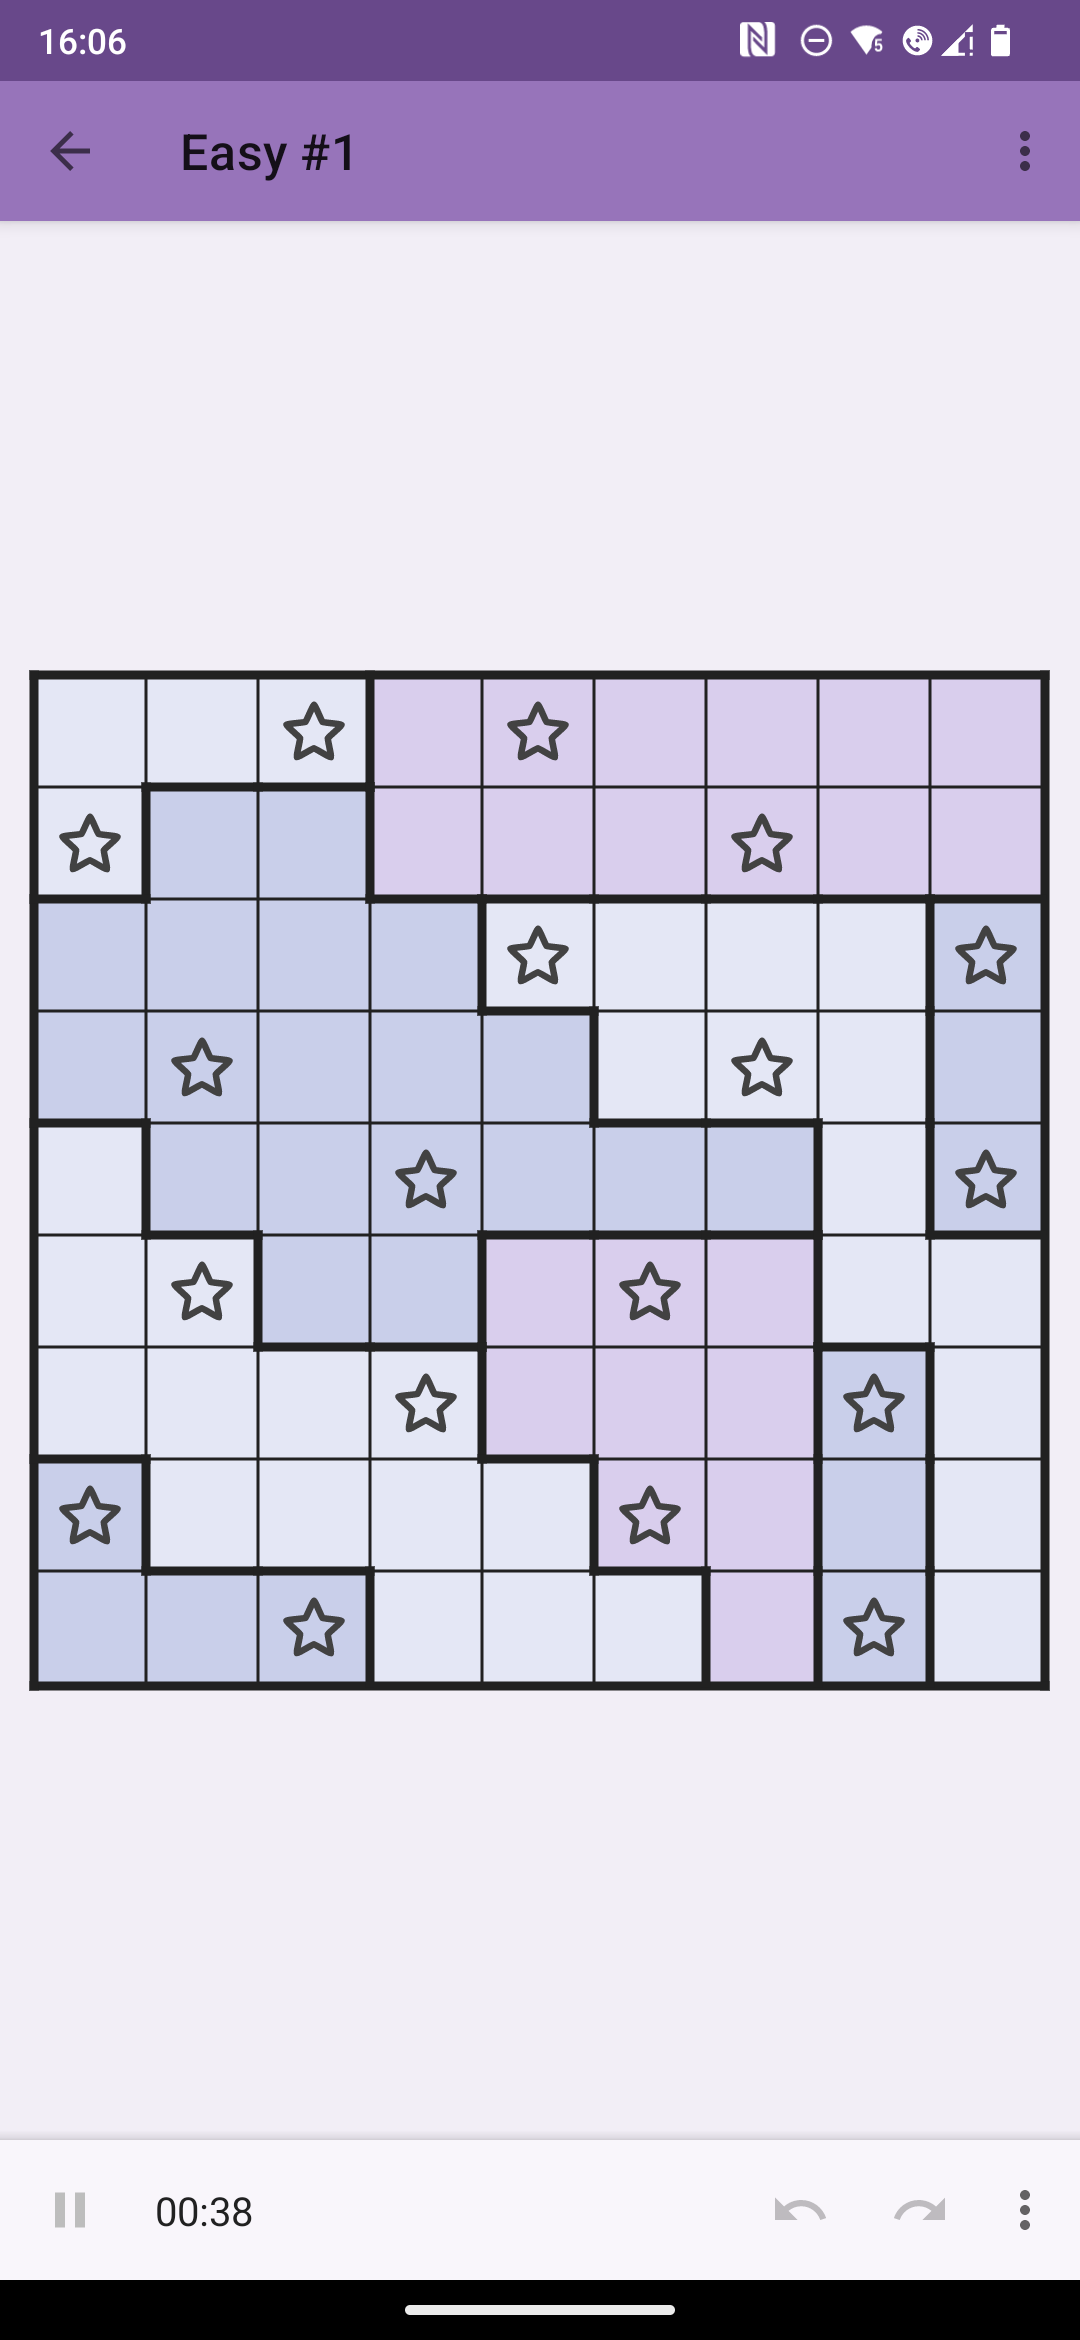
\includegraphics[height=12cm]{Easy_1_complete.png}
    \caption{An example of Star Battle puzzle in its blank state (left) and when solved (right).}\label{fig:example boards}
\end{figure}

\pagebreak
\printbibliography[heading=bibintoc, title={References}]

\end{document}